\documentclass[aspectratio=169,10pt]{beamer}
\usepackage[utf8]{inputenc}
\usepackage{amsmath, amssymb, bm, amsfonts}
\usepackage{booktabs}
\usepackage{tabularx}
\usepackage{graphicx}
\usepackage{tikz}
\usetikzlibrary{arrows.meta, positioning, calc, shapes.geometric}

% --- Search paths for logo image (root directory or Images/ subfolder) ---
\graphicspath{{./}{Images/}}

% --- Universidad de Antioquia (UdeA) Custom Theme Setup ---
\definecolor{UdeAGreen}{HTML}{006241}
\definecolor{UdeAGreenDark}{HTML}{004d33}
\definecolor{UdeAGreenLight}{HTML}{007850}
\definecolor{UdeAGold}{HTML}{D4AF37}
\definecolor{Charcoal}{HTML}{2B2B2B}
\definecolor{LightBg}{HTML}{F8F9FA}

% --- THEME AND FONT ---
\usetheme{Madrid}
\usefonttheme{professionalfonts}

% Palette setup matching the 3-tone green infolines footer and header
\setbeamercolor{palette primary}{bg=UdeAGreenDark, fg=white}
\setbeamercolor{palette secondary}{bg=UdeAGreenLight, fg=white}
\setbeamercolor{palette tertiary}{bg=UdeAGreen, fg=white}
\setbeamercolor{structure}{fg=UdeAGreen}
\setbeamercolor{background canvas}{bg=LightBg}
\setbeamercolor{text}{fg=Charcoal}

% --- Block Style Customization ---
\setbeamercolor{block title}{bg=UdeAGreen, fg=white}
\setbeamercolor{block body}{bg=white, fg=Charcoal}
\setbeamercolor{block title example}{bg=UdeAGold, fg=Charcoal}
\setbeamercolor{block body example}{bg=white, fg=Charcoal}
\setbeamercolor{block title alert}{bg=red!75!black, fg=white}
\setbeamercolor{block body alert}{bg=white, fg=Charcoal}

\setbeamertemplate{navigation symbols}{}

% --- LOGO CONFIGURATION ---
% 1. Logo on following slides: placed automatically in the bottom-right corner above the footer
\logo{
\includegraphics[width=1.15cm]{UdeA+simplificado+Negro_Smaller.png}}

% 2. Logo on title slide: centered below the date
\titlegraphic{\vspace{0.15cm}
\includegraphics[width=2.8cm]{UdeA+simplificado+Negro_Smaller.png}}

% --- PRESENTATION METADATA ---
\title[PhD Research Proposal]{Forecasting Catastrophic Scenarios in LEO via Symplectic N-Body Integrators}
\subtitle{AI-Enhanced Hybrid Framework for Massive Space Debris Population Dynamics}
\author[J. F. Puerta-Ibarra (Aerospace Engineering)]{Juan Francisco Puerta-Ibarra}
\institute[Aerospace Engineering]{Faculty of Engineering \\ Universidad de Antioquia}
\date[Doctoral Defense]{Doctoral Research}

\begin{document}

% ==============================================================================
% SLIDE 1: TITLE SLIDE (Centered Logo via \titlegraphic)
% ==============================================================================
\begin{frame}[plain]
    \titlepage
\end{frame}

% ==============================================================================
% SLIDE 2: ROADMAP
% ==============================================================================
\begin{frame}{Research Questions and Presentation Roadmap}
    \begin{columns}[t]
        \begin{column}{0.31\textwidth}
            \begin{block}{\textbf{Question 1: Current State}}
                \small
                \textbf{What has been done} regarding LEO catastrophic scenario forecasting using symplectic N-body integrators?
                \begin{itemize}
                    \setlength{\itemsep}{2pt}
                    \item Classical Solar System tools
                    \item The LEO dissipative barrier
                    \item Preliminary AAS 25-787 core
                \end{itemize}
            \end{block}
        \end{column}
        
        \begin{column}{0.31\textwidth}
            \begin{exampleblock}{\textbf{Question 2: Gaps and Ideas}}
                \small
                \textbf{What could be done} to improve state-of-the-art modeling and resolve runtime bottlenecks?
                \begin{itemize}
                    \setlength{\itemsep}{2pt}
                    \item PINN atmospheric models
                    \item Multi-node GPU scaling
                    \item Backward RL time-inversion
                \end{itemize}
            \end{exampleblock}
        \end{column}
        
        \begin{column}{0.31\textwidth}
            \begin{alertblock}{\textbf{Question 3: Thesis Plan}}
                \small
                \textbf{What should be done} to fulfill the doctoral objectives and validate deliverables?
                \begin{itemize}
                    \setlength{\itemsep}{2pt}
                    \item 6 Specific work packages
                    \item Quantitative error metrics
                    \item 24-Month execution plan
                \end{itemize}
            \end{alertblock}
        \end{column}
    \end{columns}
\end{frame}

% ==============================================================================
% SLIDE 3: QUESTION 1 - SOTA
% ==============================================================================
\begin{frame}{Question 1: State of the Art in Symplectic LEO Propagation}
    \begin{columns}[t]
        \begin{column}{0.48\textwidth}
            \begin{block}{Traditional Astrodynamics Framework}
                \small
                \begin{itemize}
                    \setlength{\itemsep}{3pt}
                    \item \textbf{Planetary Domain:} Symplectic schemes (WHFast, Wisdom-Holman) preserve phase-space volume ($d\mathbf{p} \wedge d\mathbf{q}$) over $10^6$ orbits in conservative fields.
                    \item \textbf{LEO Dissipative Barrier:} Symplectic invariants break under non-conservative atmospheric drag and solar radiation pressure (SRP).
                    \item \textbf{Standard Workarounds:} Classical tools (NASA GMAT, STK, Cowell/RK8) compute drag accurately, but suffer severe accumulated truncation error and prohibitive $O(N^2)$ costs for $N > 10^4$.
                \end{itemize}
            \end{block}
        \end{column}

        \begin{column}{0.48\textwidth}
            \begin{exampleblock}{Debris Clouds and Integration Extensions}
                \small
                \begin{itemize}
                    \setlength{\itemsep}{3pt}
                    \item \textbf{Breakup Models:} NASA EVOLVE 4.0 and ESA models statistically predict fragment size, mass, and velocity spreads.
                    \item \textbf{REBOUNDx Extension:} Operator-splitting enables dissipative forces, but typically lacks specialized geopotential-drag balance for LEO.
                    \item \textbf{Statistical Collision Proxies:} Density-based methods estimate collision rates, but miss individual deterministic orbital conjunctions.
                \end{itemize}
            \end{exampleblock}
        \end{column}
    \end{columns}
\end{frame}

% ==============================================================================
% SLIDE 4: QUESTION 1 - PRELIMINARY BENCHMARKS
% ==============================================================================
\begin{frame}{Question 1: Candidate's Preliminary Achievements (AAS 25-787)}
    \begin{columns}[t]
        \begin{column}{0.48\textwidth}
            \begin{block}{Validated Hybrid Semi-Symplectic Core}
                \small
                \begin{itemize}
                    \setlength{\itemsep}{3pt}
                    \item Coupled the high-speed C core of \textbf{REBOUND} with an adapted \textbf{WHFast} integrator for low Earth orbits.
                    \item Resolved non-conservative dissipation using a \textbf{2nd-order Strang splitting} scheme separating Hamiltonian flow from drag kicks.
                    \item Benchmarked against high-fidelity numerical models, achieving sub-kilometer position consistency over 24-hour arcs.
                \end{itemize}
            \end{block}
        \end{column}

        \begin{column}{0.48\textwidth}
            \begin{block}{AAS 25-787 Quantitative Benchmarks}
                \small
                \begin{itemize}
                    \setlength{\itemsep}{3pt}
                    \item \textbf{Massive Scale:} Propagated a synthetic cloud of \textbf{20,000 autonomous fragments} simultaneously.
                    \item \textbf{Energy Conservation:} Bounded relative energy error to:
                    $$\left| \Delta E / E_0 \right| \in [10^{-8}, 10^{-7}]$$
                    \item \textbf{Nodal Precession:} Secular nodal drift matched analytical $J_2$ theory within \textbf{0.005\%} relative error.
                    \item \textbf{Speed:} Significantly outperformed classical Cowell-type explicit integrators.
                \end{itemize}
            \end{block}
        \end{column}
    \end{columns}
\end{frame}

% ==============================================================================
% SLIDE 5: STRANG SPLITTING DIAGRAM
% ==============================================================================
\begin{frame}{The Hybrid Semi-Symplectic Architecture (Strang Splitting)}
    \centering
    \resizebox{0.95\textwidth}{!}{
    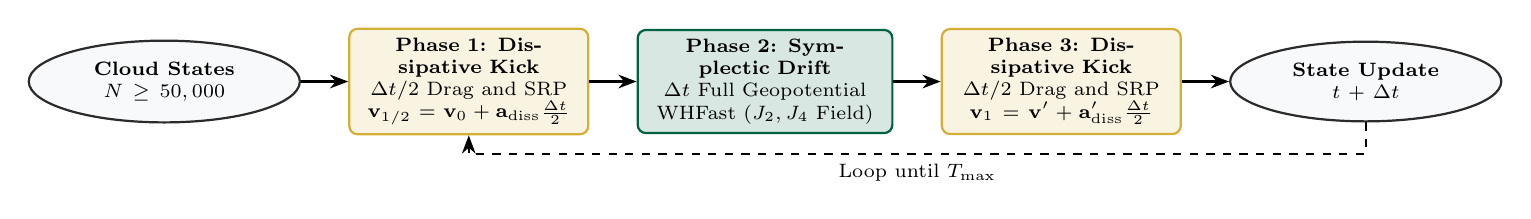
\begin{tikzpicture}[>=Stealth, auto, node distance=0.8cm]
        \tikzstyle{io}    = [ellipse, draw=Charcoal, fill=LightBg, text width=2.2cm, minimum height=0.9cm, align=center, font=\scriptsize\bfseries, thick]
        \tikzstyle{kick}  = [rectangle, draw=UdeAGold, fill=UdeAGold!15, rounded corners=3pt, text width=2.8cm, minimum height=1.1cm, align=center, font=\scriptsize, thick]
        \tikzstyle{drift} = [rectangle, draw=UdeAGreen, fill=UdeAGreen!15, rounded corners=3pt, text width=3.0cm, minimum height=1.1cm, align=center, font=\scriptsize, thick]

        % Horizontal Pipeline
        \node[io] (start) {Cloud States\\ $N \ge 50,000$};
        \node[kick, right=0.6cm of start] (k1) {\textbf{Phase 1: Dissipative Kick}\\ $\Delta t/2$ Drag and SRP\\ $\mathbf{v}_{1/2} = \mathbf{v}_0 + \mathbf{a}_{\text{diss}}\frac{\Delta t}{2}$};
        \node[drift, right=0.6cm of k1] (drift) {\textbf{Phase 2: Symplectic Drift}\\ $\Delta t$ Full Geopotential\\ WHFast ($J_2, J_4$ Field)};
        \node[kick, right=0.6cm of drift] (k2) {\textbf{Phase 3: Dissipative Kick}\\ $\Delta t/2$ Drag and SRP\\ $\mathbf{v}_1 = \mathbf{v}' + \mathbf{a}'_{\text{diss}}\frac{\Delta t}{2}$};
        \node[io, right=0.6cm of k2] (output) {State Update\\ $t + \Delta t$};

        % Arrows
        \draw[->, thick] (start) -- (k1);
        \draw[->, thick] (k1) -- (drift);
        \draw[->, thick] (drift) -- (k2);
        \draw[->, thick] (k2) -- (output);
        \draw[->, thick, dashed] (output.south) -- ++(0,-0.4) -| node[pos=0.25, below, font=\scriptsize] {Loop until $T_{\text{max}}$} (k1.south);
    \end{tikzpicture}
    }

    \vspace{0.25cm}
    \begin{alertblock}{Mathematical Flow Operator}
        \small
        $$\Phi(\Delta t) \approx \Phi_P\left(\frac{\Delta t}{2}\right) \circ \Phi_G(\Delta t) \circ \Phi_P\left(\frac{\Delta t}{2}\right) \quad \implies \quad \mathcal{O}(\Delta t^2) \text{ Accuracy with Preserved Invariants}$$
    \end{alertblock}
\end{frame}

% ==============================================================================
% SLIDE 6: QUESTION 2 - WHAT COULD BE DONE
% ==============================================================================
\begin{frame}{Question 2: Gaps and Frontiers in Long-Term LEO Forecasting}
    \begin{columns}[t]
        \begin{column}{0.48\textwidth}
            \begin{block}{1. Physics and Computational Frontiers}
                \small
                \textbf{Dynamic Atmospheric Coupling:}
                \begin{itemize}
                    \setlength{\itemsep}{2pt}
                    \item Replace static exponential density models with \textbf{Physics-Informed Neural Networks (PINNs)} or fast surrogates of NRLMSISE-00.
                    \item Reflect solar cycles ($F_{10.7}$) and geomagnetic storms ($K_p/A_p$) at high speed without stalling the integrator.
                \end{itemize}
                \vspace{0.12cm}
                \textbf{Massive Multi-Node HPC Scaling:}
                \begin{itemize}
                    \setlength{\itemsep}{2pt}
                    \item Migrate from shared-memory OpenMP to distributed multi-node GPU clusters (MPI + CUDA).
                    \item Scale simulation capacity to $>100,000$ particles to track full mega-constellation fragmentations.
                \end{itemize}
            \end{block}
        \end{column}

        \begin{column}{0.48\textwidth}
            \begin{exampleblock}{2. Temporal Inversion and AI Screening}
                \small
                \textbf{Temporal Inversion (Backward Propagation):}
                \begin{itemize}
                    \setlength{\itemsep}{2pt}
                    \item Capitalize on the geometric time-reversibility of symplectic maps.
                    \item Train a \textbf{Backward Reinforcement Learning (RL)} agent to reverse drag dissipation, pinpointing parent bodies and breakup epochs.
                \end{itemize}
                \vspace{0.12cm}
                \textbf{AI-Driven Conjunction Screening:}
                \begin{itemize}
                    \setlength{\itemsep}{2pt}
                    \item Replace costly $O(N^2)$ brute-force distance checks with \textbf{Spatio-Temporal Transformers / LSTMs}.
                    \item Rapidly project catastrophic cascade triggers (Kessler Syndrome) across 50--100 year windows.
                \end{itemize}
            \end{exampleblock}
        \end{column}
    \end{columns}
\end{frame}

% ==============================================================================
% SLIDE 7: QUESTION 3 - OBJECTIVES 1 & 2
% ==============================================================================
\begin{frame}{Question 3: Specific Objectives and Quantitative Benchmarks}
    \begin{block}{General Doctoral Objective}
        \small
        Develop, validate, and scale an AI-enhanced, hybrid semi-symplectic computational framework capable of deterministic multi-decade forecasting of massive debris clouds ($N \ge 50,000$) in perturbed LEO.
    \end{block}

    \vspace{0.1cm}

    \begin{columns}[t]
        \begin{column}{0.48\textwidth}
            \begin{exampleblock}{Specific Objective 1: Integrator Core}
                \small
                \begin{itemize}
                    \setlength{\itemsep}{2pt}
                    \item Implement a production-grade Strang splitting core in optimized C.
                    \item \textbf{Metric 1.1:} Bound numerical energy drift within $|\Delta E / E_0| \le 10^{-7}$ over long orbital arcs.
                    \item \textbf{Metric 1.2:} Keep secular nodal precession error $<0.005\%$ relative to analytical theory.
                \end{itemize}
            \end{exampleblock}
        \end{column}

        \begin{column}{0.48\textwidth}
            \begin{exampleblock}{Specific Objective 2: HPC Scalability}
                \small
                \begin{itemize}
                    \setlength{\itemsep}{2pt}
                    \item Scale parallel architecture to handle $\ge 50,000$ mutually non-interacting fragments.
                    \item \textbf{Metric 2.1:} Demonstrate linear or near-linear scaling ($O(N \log N)$ or better).
                    \item Optimize memory through pointer-aligned, cache-friendly data structures.
                \end{itemize}
            \end{exampleblock}
        \end{column}
    \end{columns}
\end{frame}

% ==============================================================================
% SLIDE 8: QUESTION 3 - OBJECTIVES 3 TO 6
% ==============================================================================
\begin{frame}{Question 3: Methodological Objectives (AI and Inversion)}
    \begin{columns}[t]
        \begin{column}{0.48\textwidth}
            \begin{block}{AI Enhancements (Specific Objs 3 and 4)}
                \small
                \textbf{PINN Thermosphere Modeling (Obj 3):}
                \begin{itemize}
                    \setlength{\itemsep}{2pt}
                    \item Train a PINN surrogate on NRLMSISE-00 / Jacchia data to capture diurnal bulges and solar flux.
                    \item Maintain $<2\%$ density discrepancy while accelerating evaluations by $>10\times$.
                \end{itemize}
                \vspace{0.12cm}
                \textbf{Conjunction Prediction (Obj 4):}
                \begin{itemize}
                    \setlength{\itemsep}{2pt}
                    \item Deploy LSTM/Transformer attention models to evaluate collision probabilities dynamically across fragment clusters.
                \end{itemize}
            \end{block}
        \end{column}

        \begin{column}{0.48\textwidth}
            \begin{exampleblock}{Inversion and Verification (Specific Objs 5 and 6)}
                \small
                \textbf{Backward RL Inversion (Obj 5):}
                \begin{itemize}
                    \setlength{\itemsep}{2pt}
                    \item Invert dissipative decay trajectories via time-reversed Strang flows.
                    \item Train an RL agent to recover fragmentation epochs ($t_0$) and parent orbits within narrow covariance bounds.
                \end{itemize}
                \vspace{0.12cm}
                \textbf{Cross-Tool Validation (Obj 6):}
                \begin{itemize}
                    \setlength{\itemsep}{2pt}
                    \item Benchmark multi-year orbital histories against \textbf{NASA GMAT (vR2025a)}, \textbf{ESA GODOT}, and \textbf{STK}.
                    \item Deliver a validated open-source C/Python library.
                \end{itemize}
            \end{exampleblock}
        \end{column}
    \end{columns}
\end{frame}

% ==============================================================================
% SLIDE 9: CHRONOGRAM
% ==============================================================================
\begin{frame}{Question 3: 24-Month Chronogram and Milestone Matrix}
    \begin{table}
        \centering
        \scriptsize
        \begin{tabularx}{\textwidth}{Xcccccc}
            \toprule
            \textbf{Research Phase / Work Package} & \textbf{M1--M4} & \textbf{M5--M8} & \textbf{M9--M12} & \textbf{M13--M16} & \textbf{M17--M20} & \textbf{M21--M24} \\
            \midrule
            1. Strang Splitting Integration Core & \textbf{X} & & & & & \\
            2. High-Performance Scaling ($\ge 50\text{k}$ particles) & & \textbf{X} & & & & \\
            3. PINN Thermospheric Surrogate Training & & & \textbf{X} & & & \\
            4. Conjunction Transformer/LSTM Logic & & & & \textbf{X} & & \\
            5. Backward RL Path Reconstruction & & & & & \textbf{X} & \\
            6. Cross-Validation (GMAT/GODOT) and Defense & & & & & & \textbf{X} \\
            \bottomrule
        \end{tabularx}
        \caption{Phased Execution Roadmap across the 2-Year Doctoral Timeline.}
    \end{table}

    \vspace{-0.1cm}
    \begin{block}{Computing Resources}
        \footnotesize
        Simulations and surrogate network training utilize the high-performance computing clusters and aerospace laboratory infrastructure of the \textbf{Faculty of Engineering at Universidad de Antioquia}.
    \end{block}
\end{frame}

% ==============================================================================
% SLIDE 10: SYNTHESIS
% ==============================================================================
\begin{frame}{Synthesis: Impact on LEO Space Sustainability}
    \begin{columns}[t]
        \begin{column}{0.31\textwidth}
            \begin{block}{What is Done}
                \small
                \begin{itemize}
                    \setlength{\itemsep}{2pt}
                    \item Validated hybrid semi-symplectic engine using 2nd-order Strang splitting.
                    \item Simulated 20,000 fragments with energy error $|\Delta E/E_0| \le 10^{-7}$ and sub-km accuracy.
                \end{itemize}
            \end{block}
        \end{column}

        \begin{column}{0.31\textwidth}
            \begin{exampleblock}{What Can Be Done}
                \small
                \begin{itemize}
                    \setlength{\itemsep}{2pt}
                    \item Introduce dynamic PINN thermosphere models.
                    \item Scale to $N \ge 50,000$ on GPU/MPI architectures.
                    \item Use time-reversibility for parent-body origin recovery.
                \end{itemize}
            \end{exampleblock}
        \end{column}

        \begin{column}{0.31\textwidth}
            \begin{alertblock}{What Will Be Done}
                \small
                \begin{itemize}
                    \setlength{\itemsep}{2pt}
                    \item Deliver 6 planned work packages over 24 months.
                    \item Model 50--100 year Kessler cascading scenarios.
                    \item Publish an open-source C/Python LEO library.
                \end{itemize}
            \end{alertblock}
        \end{column}
    \end{columns}

    \vspace{0.25cm}
    \centering
    \footnotesize
    \textbf{\textcolor{UdeAGreen}{Universidad de Antioquia -- Aerospace Engineering Research Group}} \\
    Contact: \texttt{juanf.puerta@udea.edu.co}
\end{frame}

\end{document}